\documentclass[conference,compsoc]{IEEEtran}
% Some/most Computer Society conferences require the compsoc mode option,
% but others may want the standard conference format.
%
% If IEEEtran.cls has not been installed into the LaTeX system files,
% manually specify the path to it like:
% \documentclass[conference,compsoc]{../sty/IEEEtran}

\usepackage{xcolor}
\newcommand\notes[1]{\textcolor{red}{#1}}

% Some very useful LaTeX packages include:
% (uncomment the ones you want to load)


% *** MISC UTILITY PACKAGES ***
%
%\usepackage{ifpdf}
% Heiko Oberdiek's ifpdf.sty is very useful if you need conditional
% compilation based on whether the output is pdf or dvi.
% usage:
% \ifpdf
%   % pdf code
% \else
%   % dvi code
% \fi
% The latest version of ifpdf.sty can be obtained from:
% http://www.ctan.org/pkg/ifpdf
% Also, note that IEEEtran.cls V1.7 and later provides a builtin
% \ifCLASSINFOpdf conditional that works the same way.
% When switching from latex to pdflatex and vice-versa, the compiler may
% have to be run twice to clear warning/error messages.






% *** CITATION PACKAGES ***
%
\ifCLASSOPTIONcompsoc
  % IEEE Computer Society needs nocompress option
  % requires cite.sty v4.0 or later (November 2003)
  \usepackage[nocompress]{cite}
\else
  % normal IEEE
  \usepackage{cite}
\fi
% cite.sty was written by Donald Arseneau
% V1.6 and later of IEEEtran pre-defines the format of the cite.sty package
% \cite{} output to follow that of the IEEE. Loading the cite package will
% result in citation numbers being automatically sorted and properly
% "compressed/ranged". e.g., [1], [9], [2], [7], [5], [6] without using
% cite.sty will become [1], [2], [5]--[7], [9] using cite.sty. cite.sty's
% \cite will automatically add leading space, if needed. Use cite.sty's
% noadjust option (cite.sty V3.8 and later) if you want to turn this off
% such as if a citation ever needs to be enclosed in parenthesis.
% cite.sty is already installed on most LaTeX systems. Be sure and use
% version 5.0 (2009-03-20) and later if using hyperref.sty.
% The latest version can be obtained at:
% http://www.ctan.org/pkg/cite
% The documentation is contained in the cite.sty file itself.
%
% Note that some packages require special options to format as the Computer
% Society requires. In particular, Computer Society  papers do not use
% compressed citation ranges as is done in typical IEEE papers
% (e.g., [1]-[4]). Instead, they list every citation separately in order
% (e.g., [1], [2], [3], [4]). To get the latter we need to load the cite
% package with the nocompress option which is supported by cite.sty v4.0
% and later.





% *** GRAPHICS RELATED PACKAGES ***
%
\ifCLASSINFOpdf
  \usepackage[pdftex]{graphicx}
  % declare the path(s) where your graphic files are
  % \graphicspath{{../pdf/}{../jpeg/}}
  % and their extensions so you won't have to specify these with
  % every instance of \includegraphics
  % \DeclareGraphicsExtensions{.pdf,.jpeg,.png}
\else
  % or other class option (dvipsone, dvipdf, if not using dvips). graphicx
  % will default to the driver specified in the system graphics.cfg if no
  % driver is specified.
  \usepackage[dvips]{graphicx}
  % declare the path(s) where your graphic files are
  % \graphicspath{{../eps/}}
  % and their extensions so you won't have to specify these with
  % every instance of \includegraphics
  % \DeclareGraphicsExtensions{.eps}
\fi
% graphicx was written by David Carlisle and Sebastian Rahtz. It is
% required if you want graphics, photos, etc. graphicx.sty is already
% installed on most LaTeX systems. The latest version and documentation
% can be obtained at: 
% http://www.ctan.org/pkg/graphicx
% Another good source of documentation is "Using Imported Graphics in
% LaTeX2e" by Keith Reckdahl which can be found at:
% http://www.ctan.org/pkg/epslatex
%
% latex, and pdflatex in dvi mode, support graphics in encapsulated
% postscript (.eps) format. pdflatex in pdf mode supports graphics
% in .pdf, .jpeg, .png and .mps (metapost) formats. Users should ensure
% that all non-photo figures use a vector format (.eps, .pdf, .mps) and
% not a bitmapped formats (.jpeg, .png). The IEEE frowns on bitmapped formats
% which can result in "jaggedy"/blurry rendering of lines and letters as
% well as large increases in file sizes.
%
% You can find documentation about the pdfTeX application at:
% http://www.tug.org/applications/pdftex





% *** MATH PACKAGES ***
%
\usepackage{amsmath}
% A popular package from the American Mathematical Society that provides
% many useful and powerful commands for dealing with mathematics.
%
% Note that the amsmath package sets \interdisplaylinepenalty to 10000
% thus preventing page breaks from occurring within multiline equations. Use:
\interdisplaylinepenalty=2500
% after loading amsmath to restore such page breaks as IEEEtran.cls normally
% does. amsmath.sty is already installed on most LaTeX systems. The latest
% version and documentation can be obtained at:
% http://www.ctan.org/pkg/amsmath





% *** SPECIALIZED LIST PACKAGES ***
%
%\usepackage{algorithmic}
% algorithmic.sty was written by Peter Williams and Rogerio Brito.
% This package provides an algorithmic environment fo describing algorithms.
% You can use the algorithmic environment in-text or within a figure
% environment to provide for a floating algorithm. Do NOT use the algorithm
% floating environment provided by algorithm.sty (by the same authors) or
% algorithm2e.sty (by Christophe Fiorio) as the IEEE does not use dedicated
% algorithm float types and packages that provide these will not provide
% correct IEEE style captions. The latest version and documentation of
% algorithmic.sty can be obtained at:
% http://www.ctan.org/pkg/algorithms
% Also of interest may be the (relatively newer and more customizable)
% algorithmicx.sty package by Szasz Janos:
% http://www.ctan.org/pkg/algorithmicx




% *** ALIGNMENT PACKAGES ***
%
%\usepackage{array}
% Frank Mittelbach's and David Carlisle's array.sty patches and improves
% the standard LaTeX2e array and tabular environments to provide better
% appearance and additional user controls. As the default LaTeX2e table
% generation code is lacking to the point of almost being broken with
% respect to the quality of the end results, all users are strongly
% advised to use an enhanced (at the very least that provided by array.sty)
% set of table tools. array.sty is already installed on most systems. The
% latest version and documentation can be obtained at:
% http://www.ctan.org/pkg/array


% IEEEtran contains the IEEEeqnarray family of commands that can be used to
% generate multiline equations as well as matrices, tables, etc., of high
% quality.




% *** SUBFIGURE PACKAGES ***
%\ifCLASSOPTIONcompsoc
%  \usepackage[caption=false,font=footnotesize,labelfont=sf,textfont=sf]{subfig}
%\else
%  \usepackage[caption=false,font=footnotesize]{subfig}
%\fi
% subfig.sty, written by Steven Douglas Cochran, is the modern replacement
% for subfigure.sty, the latter of which is no longer maintained and is
% incompatible with some LaTeX packages including fixltx2e. However,
% subfig.sty requires and automatically loads Axel Sommerfeldt's caption.sty
% which will override IEEEtran.cls' handling of captions and this will result
% in non-IEEE style figure/table captions. To prevent this problem, be sure
% and invoke subfig.sty's "caption=false" package option (available since
% subfig.sty version 1.3, 2005/06/28) as this is will preserve IEEEtran.cls
% handling of captions.
% Note that the Computer Society format requires a sans serif font rather
% than the serif font used in traditional IEEE formatting and thus the need
% to invoke different subfig.sty package options depending on whether
% compsoc mode has been enabled.
%
% The latest version and documentation of subfig.sty can be obtained at:
% http://www.ctan.org/pkg/subfig




% *** FLOAT PACKAGES ***
%
%\usepackage{fixltx2e}
% fixltx2e, the successor to the earlier fix2col.sty, was written by
% Frank Mittelbach and David Carlisle. This package corrects a few problems
% in the LaTeX2e kernel, the most notable of which is that in current
% LaTeX2e releases, the ordering of single and double column floats is not
% guaranteed to be preserved. Thus, an unpatched LaTeX2e can allow a
% single column figure to be placed prior to an earlier double column
% figure.
% Be aware that LaTeX2e kernels dated 2015 and later have fixltx2e.sty's
% corrections already built into the system in which case a warning will
% be issued if an attempt is made to load fixltx2e.sty as it is no longer
% needed.
% The latest version and documentation can be found at:
% http://www.ctan.org/pkg/fixltx2e


%\usepackage{stfloats}
% stfloats.sty was written by Sigitas Tolusis. This package gives LaTeX2e
% the ability to do double column floats at the bottom of the page as well
% as the top. (e.g., "\begin{figure*}[!b]" is not normally possible in
% LaTeX2e). It also provides a command:
%\fnbelowfloat
% to enable the placement of footnotes below bottom floats (the standard
% LaTeX2e kernel puts them above bottom floats). This is an invasive package
% which rewrites many portions of the LaTeX2e float routines. It may not work
% with other packages that modify the LaTeX2e float routines. The latest
% version and documentation can be obtained at:
% http://www.ctan.org/pkg/stfloats
% Do not use the stfloats baselinefloat ability as the IEEE does not allow
% \baselineskip to stretch. Authors submitting work to the IEEE should note
% that the IEEE rarely uses double column equations and that authors should try
% to avoid such use. Do not be tempted to use the cuted.sty or midfloat.sty
% packages (also by Sigitas Tolusis) as the IEEE does not format its papers in
% such ways.
% Do not attempt to use stfloats with fixltx2e as they are incompatible.
% Instead, use Morten Hogholm'a dblfloatfix which combines the features
% of both fixltx2e and stfloats:
%
% \usepackage{dblfloatfix}
% The latest version can be found at:
% http://www.ctan.org/pkg/dblfloatfix




% *** PDF, URL AND HYPERLINK PACKAGES ***
%
\usepackage{url}
% url.sty was written by Donald Arseneau. It provides better support for
% handling and breaking URLs. url.sty is already installed on most LaTeX
% systems. The latest version and documentation can be obtained at:
% http://www.ctan.org/pkg/url
% Basically, \url{my_url_here}.




% *** Do not adjust lengths that control margins, column widths, etc. ***
% *** Do not use packages that alter fonts (such as pslatex).         ***
% There should be no need to do such things with IEEEtran.cls V1.6 and later.
% (Unless specifically asked to do so by the journal or conference you plan
% to submit to, of course. )


% correct bad hyphenation here
\hyphenation{op-tical net-works semi-conduc-tor}


\begin{document}
%
% paper title
% Titles are generally capitalized except for words such as a, an, and, as,
% at, but, by, for, in, nor, of, on, or, the, to and up, which are usually
% not capitalized unless they are the first or last word of the title.
% Linebreaks \\ can be used within to get better formatting as desired.
% Do not put math or special symbols in the title.
\title{Resolving Limits Faced by Classical Machine Learning Approaches:\\Areas of Application for 
Collaborative Interactive Learning Techniques}


% author names and affiliations
% use a multiple column layout for up to three different
% affiliations
\author{\IEEEauthorblockN{Christoph Sonntag$^1$}
\IEEEauthorblockA{$^1$Intelligent Systems Group, University of Passau, Innstrasse 70, Passau, Germany\\
sonntagc@fim.uni-passau.de}
}

% conference papers do not typically use \thanks and this command
% is locked out in conference mode. If really needed, such as for
% the acknowledgment of grants, issue a \IEEEoverridecommandlockouts
% after \documentclass

% for over three affiliations, or if they all won't fit within the width
% of the page (and note that there is less available width in this regard for
% compsoc conferences compared to traditional conferences), use this
% alternative format:
% 
%\author{\IEEEauthorblockN{Michael Shell\IEEEauthorrefmark{1},
%Homer Simpson\IEEEauthorrefmark{2},
%James Kirk\IEEEauthorrefmark{3}, 
%Montgomery Scott\IEEEauthorrefmark{3} and
%Eldon Tyrell\IEEEauthorrefmark{4}}
%\IEEEauthorblockA{\IEEEauthorrefmark{1}School of Electrical and Computer Engineering\\
%Georgia Institute of Technology,
%Atlanta, Georgia 30332--0250\\ Email: see http://www.michaelshell.org/contact.html}
%\IEEEauthorblockA{\IEEEauthorrefmark{2}Twentieth Century Fox, Springfield, USA\\
%Email: homer@thesimpsons.com}
%\IEEEauthorblockA{\IEEEauthorrefmark{3}Starfleet Academy, San Francisco, California 96678-2391\\
%Telephone: (800) 555--1212, Fax: (888) 555--1212}
%\IEEEauthorblockA{\IEEEauthorrefmark{4}Tyrell Inc., 123 Replicant Street, Los Angeles, California 90210--4321}}



% use for special paper notices
%\IEEEspecialpapernotice{(Invited Paper)}



% make the title area
\maketitle

% As a general rule, do not put math, special symbols or citations
% in the abstract
\begin{abstract}
The area of \textit{Machine Learning (ML)} has experienced a high 
level of research interest in the last few years with it's underlying 
theory reaching back far into the 18Th century. Due to minimal 
costs for computation and the massive availability of data in the 
Internet recent research interest has been mainly focused on 
\textit{automatic ML (aML)}. In this ML paradigm a model 
(e.g.\ classifier, \dots) is being trained with a pre-labeled training 
set in order to make predictions on unknown unlabeled data. Problems arise 
in domains where data is rarely available or where the labeling process is 
too expensive (computationally or economically). Furthermore, real-world data 
can be uncertain, incomplete or contain noisy data. In these cases 
full automation is not reliable enough or even infeasible for specific 
domains. However, robust and trustworthy results are mandatory in a lot of 
applications like health informatics or autonomous vehicles. 
Therefore, systems are needed that interactively integrate knowledge from 
various experts, which can be collaborating humans or machines, in order 
to continuously improve results over a systems whole lifetime: So called 
\textit{Collaborative Interactive Learning (CIL)} systems.
This paper contributes in presenting an overview of classical ML approaches 
in comparison with CIL and outlines possible areas of application. 
\notes{Abstract kuerzen, 18th Jahrhundert interessiert niemanden.}
\end{abstract}


\section{Introduction}
As with most concepts, there is no canonical 
definition for the term \textit{Machine Learning} but at its most basic form it 
can be described as algorithms that learn from a given set of training examples 
$\{(x_i, y_i)\}$ of inputs $x_i$ and outputs $y_i$ in order to 
make predictions on unknown input data. According to Tom 
Mitchell, a Computer Scientist from Carnegie Mellon University, ML tries 
to answer how we can build algorithms that automatically improve through 
experience and what fundamental laws govern all these learning processes\cite{ML:mitchell}.
The area of ML in general is a fast-growing discipline at the intersection of statistics 
and computer science and has experienced massive research interest in the last decades.
With its various application possibilities it has also been an interesting branch for 
economists and entrepreneurs.
Since ML scenarios like \textit{supervised}, \textit{unsupervised} and 
\textit{semi-supervised} learning, which we will cover later, are heavily data-driven, 
the Internet with its massive amount of data has contributed to the further development 
of research in the area of fully automated learning algorithms. Today, we can see the 
results in a variety of applications\cite{FoundationsOfML:mohri}\cite{DisciplineOfML:mitchell}, 
not limited to the list below.
\begin{itemize}
    \item \textit{Text classification, Natural Language Processing (NLP)}. 
        Many current mail programs have built-in spam detection which originally used
        simple regular expressions in order to detect phrases commonly used in spam mails.
        With state-of-the-art ML techniques it is not only possible for a mail program to 
        query for a number of words but to the pattern how spam mails are constructed and 
        to adapt itself to new types of spam.
    \item \textit{Speech recognition}. 
        Most commercial applications for speech recognition use ML to train itself to 
        recognize a users speech input. \notes{Umformen. Beschreiben, wofür ML genutzt wird.}
    \item \textit{Image recognition, OCR}.
        Machine Learning methods have also been successfully applied in domains where it's 
        important to extract information from images such as detecting and classifiying 
        objects or recognize handwritten \notes{only handwritten?} characters. Image 
        recognition and OCR are therefore for example used in medical diagnosis to 
        detect cancer on radiographs, in autonomous vehicles to detect obstacles and to 
        stay on track or in post-offices to sort envelopes with hand-written addresses. 
        \notes{Nochmal eine Quellenangabe?}
    \item \textit{Games}.
        Computer Games ususally offer a Multiplayer mode where a user can interact and 
        play the game even without a human opponent. For games with a small number of 
        possible moves after each turn, and therefore a realtively small game tree conatining 
        all possible moves, the minimax algorithm\cite{Prog2:bachmaier} can be sufficient. 
        It figures out which next move would minimize the worst-case scenario for all subsequent 
        moves. Therefore, it needs to know all possible moves, which can easily be computationally 
        infeasible for games like Chess or AlphaGo where a general move faces between 35 (Chess) and 
        250 (AlphaGo) possible subsequent game states.
        In order to still have challenging opponents modern Games are using ML to gain experience 
        by themselves.
    \item \textit{Search engines, Recommendation systems}.
        Nearly all current search machines use ML in one fashion or another. They mainly use these 
        techniques for \textit{(1) User classification}\notes{[q?]} in order to offer personalized 
        search results and for \textit{(2) Query classification} in order to ``understand' a 
        users query and to provide further meaningful information.
\end{itemize}

Despite the successfull application of ML in a lot of fields, most of these examples 
need a sufficient amount of labeled training data ($x_i$ with assigned $y_i$) in order to make 
correct predictions on or discover structured patterns in unknown data $x_j$. However, most 
data sets in the biomedical domain, in robotics or in other fields, where data is collected 
from sensor systems or other unreliable sources, are often either not available (e.g.\ rare 
diseases, borderline cases in road traffic, \dots) or contain noisy data, dirty data or unwanted 
data due to dirty sensors or poor visibility conditions in camera applications.
In addition, a machine learning algorithms prediction is solely based on the training data it 
has seen before. One might argue, that human decisions are also only based on experience they have 
made since their childhood but humans are often still superior to most algorithms in terms of 
the instinctive interpretation of complex patterns. Furthermore, they can learn to recognize 
structural patterns from very few training data.

\begin{figure}[!h]
\centering
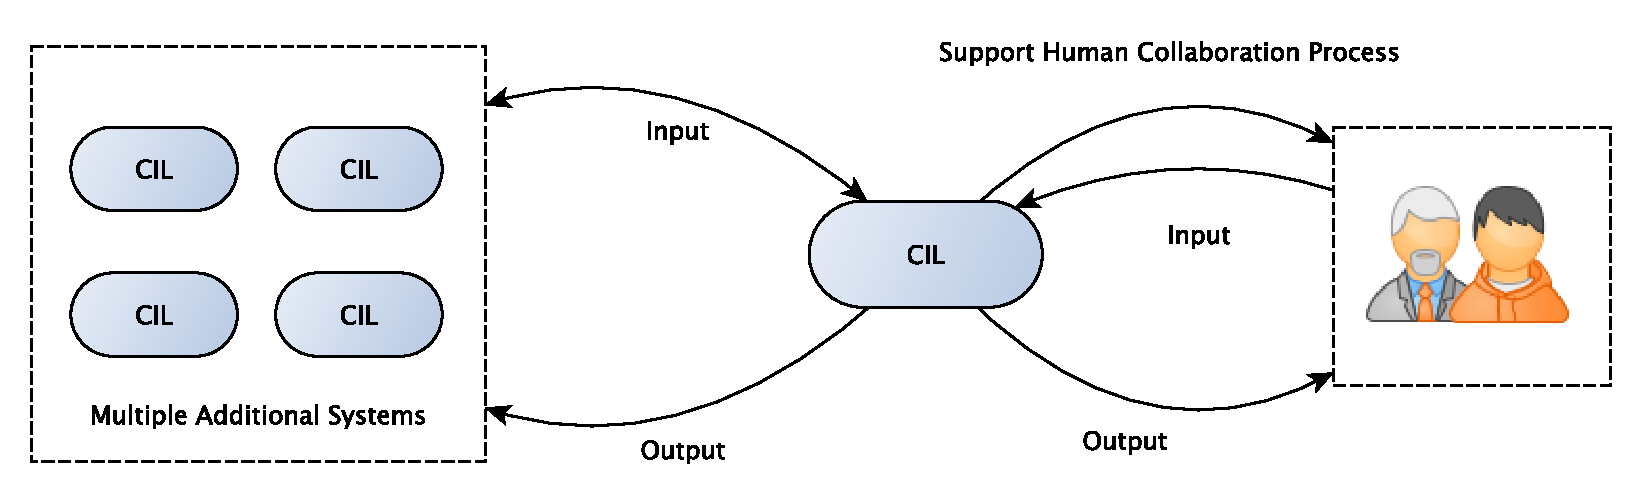
\includegraphics[width=3.5in]{images/CIL}
\caption{Collaborative Interactive Learning.}
\label{fig:CIL}
\end{figure}

Hence, \textit{Collaborative Interactive Learning (CIL)} includes domain experts (humans) 
and other CIL systems in the decision/prediction making process as shown in 
Figure~\ref{fig:CIL}. The relatively new term describes a new 
generation of systems with
\begin{itemize}
    \item lifelong learning capabilities in order to continuously improve its 
        knowledge base
    \item and the ability to exchange knowledge with other CIL systems as well as humans 
        in order to improve the own knowledge and the one of other entities in a 
        bi-directional way\cite{CIL:sick}.
\end{itemize}

This article gives a brief introduction on possible areas of application for the CIL-approach. 
It starts with an overview of classical machine learning scenarios, discussing where they are 
facing limits and motivating the use of CIL\@. It then lists possble applications and concludes 
with a view on future research interests.\notes{Relation to Organic Computing?}


\section{Algorithmic Foundations}
Bevor wir uns genauer den Anwendungen und Herausforderungen von CIL widmen, schauen wir uns 
zuerst vorhandene machine learning Strategien und Algorithmen an. Wie oben bereits angedeutet, 
gibt es eine Vielzahl an Definitionen für den Begriff ML\@. Hauptsächlich hat jedoch Arthur Samuel 
diesen Begriff im Jahr 1959 geprägt. Seitdem hat sich in diesem Bereich natürlich einiges geändert, 
jedoch gilt die Definition, dass ML Computern erlaubt Probleme zu lösen, ohne speziell dafür 
programmiert zu sein, heute immer noch\cite{MLStudiesUsingCheckers:samuel}.

Über die letzten Jahrzehnte hat sich ML stark weiterentwickelt und ist zu einem Bereich 
starken Forschungsinteresse vieler verschiedener Akteure geworden, was es schwierig macht, 
Lern-Strategien in verschiedene Kategorien einzuteilen. Unterschiedliche Forscher nutzen 
dazu verschiedene Ansätze\cite{FoundationsOfML:mohri}\cite{Structure:corne}. Im folgenden 
wollen wir fünf Strategien vorstellen\cite{FoundationsOfML:mohri}.

\subsection{Supervised learning}
Basically supervised learning is the way of learning from labeled examples and making predictions 
for all unseen points. This is the most basic concept of ML and used in a variety of applications 
where labeled data is easy to obtain. The spam mail example discussed in the introduction is an 
instance of supervised learning.

\subsection{Unsupervised learning}
Im Gegensatz zu supervised learning erhält der Lernende mit dieser Technik ausschließlich 
unlabeled training data und macht Vorraussagen für alle ungesehene Punkte. Diese Technik ist 
relativ ähnlich zu der Art, wie Säuglinge neue Sachen lernen (Lernen von Sprache) und 
findet zum Beispiel Einsatz im Clustering von Daten in Gruppen\cite{BrainInf:holzinger}.

\subsection{Semi-supervised learning}
Wie der Name suggeriert erhält der Lernende bei dieser Technik Trainingsdaten, die sowohl aus 
labeled als auch aus unlabeled data besteht und macht Vorraussagen für alle ungesehenen Punkte.
Diese Technik wird hauptsählich in Bereichen eingesetzt, in denen Daten leicht zu erreichen sind, 
aber das finden von passenden Labels teuer ist.

\subsection{Reinforcement Learning}\label{reinforcement}
Reinforcement Learning ist der wohl älteste Ansatz und ein potentiell wichtiger Ansatz für CIL\@. 
Der Lernende interagiert mit seiner Umgebung, um neue Informationen zu gewinnen. Für jede Aktion 
erhält er eine Belohnung. Sein Ziel ist es über mehrere Wiederholungen seine Belohnung zu 
maximieren. Er befindet sich so jedoch im Zwiespalt zwischen der Entscheidung bereits gewonnene 
Information auszunutzen oder mehr Informationen durch weiter Aktionen zu erhalten.

\subsection{Active Learning}\label{active}
Das Ziel von Active Learning ist es, durch geschicktes interaktives Agieren mit anderen Agenten 
bereits vorhandene Datenpunkte zu beschriften und so eine ähnliche Performance bei weniger 
Informationen zu erreichen, wie in der Methode des supervised learning. Um das zu erreichen, 
benötigt der Lernende eine Auswahlstrategie\cite{ActiveToDedicated:calma}, die entscheidet ob 
eine Aktion einen ausreichend großen für das beschriften eines Datenpunkts bringt oder nicht.

\section{When is using CIL helpful?}\label{AdvantageOfCIL}
In etablierten ML Systemen muss für jede spezielle Anwendung ein eigenes Modell im Voraus 
entworfen und trainiert werden. ML Systeme haben also einen relativ schmalen Anwendungsrahmen. 
Die Idee bei CIL-Systemen ist, dass sie ein Leben lang lernen und selbstorganisiert Wissen 
aus verschiedenen Quellen sammeln und auswerten, um so gemeinsam mit anderen technischen 
und menschlichen Agenten kollaborierend und austauschend Probleme lösen\cite{CIL:sick}. 
Der CIL-Ansatz integriert also ganz bewusst andere intelligente Systeme 
(Menschen und Maschinen) in den Entscheidungsprozess, um für die einzelnen Entitäten 
ansonsten schwierige Probleme einfacher zu lösen.
Ein weiterer Unterschied zu klassischen Ansätzen stellt der wechselseitig Nutzen dar. 
Maschinen profitieren nicht nur von Trainingsdaten anderer Agenten, sondern leisten 
einen eigenen Beitrag, um Kollaborationsprozesse von Menschen aktiv zu unterstützen, indem 
sie ihre Wünsche und Bedürfnisse erkennen und entsprechend reagieren\cite{CIL:sick}.
\notes{D-CIL und O-CIL, obwohl man unterscheidet, betrachten wir hier nur allgemeines Modell.}

\section{Classification of CIL in Organic Computing}
CIL-Systeme können sozusagen teilweise als organisch strukturierte Informationstechnologie verstanden 
werden, die sogenannte Selbst-x-Eigenschaften erfüllen\cite{Organic:schloer}\cite{Organic:schmeck}, 
sich also 
\begin{itemize}
    \item selbst konfigurieren, in dem Sinn, dass sie nicht von Entwicklern auf einen 
        Anwendungsfall ausgerichtet werden, 
    \item selbst optimieren, indem sie verschiedene Strategien des ML anwenden, um ihr 
        Wissen zu erweitern, 
    \item und sich selbst heilen und schützen, da Kooperation mit anderen System möglich ist.
\end{itemize}
Je nachdem welche Methoden des ML eingesetzt werden, sind CIL-Systeme in der Entwicklung auch 
mehr oder weniger selbst erklärend\cite{Organic:schloer}.

\section{Application examples}
\subsection{Clustering}


\subsection{Health Domain}


\subsection{Industry and Manufacturing}


\subsection{Agriculture}


\begin{itemize}
    \item Clustering
        \begin{itemize}
            \item (clustering communities on Facebook for group target advertising (politics))
            \item Methods: k-Means, DJ-clustering? --> add paper ref
        \end{itemize}
    \item Health
        \begin{itemize}
            \item Detecting cancer on radon, Prof. Sauer/Forwiss research?
            \item Growing number of users are using smartphones sensors and related devices for 
                collating a range of health information, track regularly and detect patterns (noise?, privacy?)
        \end{itemize}
    \item Industry and Manufacturing
        \begin{itemize}
            \item quality assurance
        \end{itemize}
    \item Agriculture
        \begin{itemize}
            \item Detecting bad grains, $\rightarrow$ Hackzurich project
        \end{itemize}
\end{itemize}


\section{Limitations/Challenges}
Challenges


\section{Conclusion/Future Directions}
The conclusion goes here.


% An example of a floating figure using the graphicx package.
% Note that \label must occur AFTER (or within) \caption.
% For figures, \caption should occur after the \includegraphics.
% Note that IEEEtran v1.7 and later has special internal code that
% is designed to preserve the operation of \label within \caption
% even when the captionsoff option is in effect. However, because
% of issues like this, it may be the safest practice to put all your
% \label just after \caption rather than within \caption{}.
%
% Reminder: the "draftcls" or "draftclsnofoot", not "draft", class
% option should be used if it is desired that the figures are to be
% displayed while in draft mode.
%
%\begin{figure}[!t]
%\centering
%\includegraphics[width=2.5in]{myfigure}
% where an .eps filename suffix will be assumed under latex, 
% and a .pdf suffix will be assumed for pdflatex; or what has been declared
% via \DeclareGraphicsExtensions.
%\caption{Simulation results for the network.}
%\label{fig_sim}
%\end{figure}

% Note that the IEEE typically puts floats only at the top, even when this
% results in a large percentage of a column being occupied by floats.


% An example of a double column floating figure using two subfigures.
% (The subfig.sty package must be loaded for this to work.)
% The subfigure \label commands are set within each subfloat command,
% and the \label for the overall figure must come after \caption.
% \hfil is used as a separator to get equal spacing.
% Watch out that the combined width of all the subfigures on a 
% line do not exceed the text width or a line break will occur.
%
%\begin{figure*}[!t]
%\centering
%\subfloat[Case I]{\includegraphics[width=2.5in]{box}%
%\label{fig_first_case}}
%\hfil
%\subfloat[Case II]{\includegraphics[width=2.5in]{box}%
%\label{fig_second_case}}
%\caption{Simulation results for the network.}
%\label{fig_sim}
%\end{figure*}
%
% Note that often IEEE papers with subfigures do not employ subfigure
% captions (using the optional argument to \subfloat[]), but instead will
% reference/describe all of them (a), (b), etc., within the main caption.
% Be aware that for subfig.sty to generate the (a), (b), etc., subfigure
% labels, the optional argument to \subfloat must be present. If a
% subcaption is not desired, just leave its contents blank,
% e.g., \subfloat[].


% An example of a floating table. Note that, for IEEE style tables, the
% \caption command should come BEFORE the table and, given that table
% captions serve much like titles, are usually capitalized except for words
% such as a, an, and, as, at, but, by, for, in, nor, of, on, or, the, to
% and up, which are usually not capitalized unless they are the first or
% last word of the caption. Table text will default to \footnotesize as
% the IEEE normally uses this smaller font for tables.
% The \label must come after \caption as always.
%
%\begin{table}[!t]
%% increase table row spacing, adjust to taste
%\renewcommand{\arraystretch}{1.3}
% if using array.sty, it might be a good idea to tweak the value of
% \extrarowheight as needed to properly center the text within the cells
%\caption{An Example of a Table}
%\label{table_example}
%\centering
%% Some packages, such as MDW tools, offer better commands for making tables
%% than the plain LaTeX2e tabular which is used here.
%\begin{tabular}{|c||c|}
%\hline
%One & Two\\
%\hline
%Three & Four\\
%\hline
%\end{tabular}
%\end{table}


% Note that the IEEE does not put floats in the very first column
% - or typically anywhere on the first page for that matter. Also,
% in-text middle ("here") positioning is typically not used, but it
% is allowed and encouraged for Computer Society conferences (but
% not Computer Society journals). Most IEEE journals/conferences use
% top floats exclusively. 
% Note that, LaTeX2e, unlike IEEE journals/conferences, places
% footnotes above bottom floats. This can be corrected via the
% \fnbelowfloat command of the stfloats package.


% trigger a \newpage just before the given reference
% number - used to balance the columns on the last page
% adjust value as needed - may need to be readjusted if
% the document is modified later
%\IEEEtriggeratref{8}
% The "triggered" command can be changed if desired:
%\IEEEtriggercmd{\enlargethispage{-5in}}

% references section

% can use a bibliography generated by BibTeX as a .bbl file
% BibTeX documentation can be easily obtained at:
% http://mirror.ctan.org/biblio/bibtex/contrib/doc/
% The IEEEtran BibTeX style support page is at:
% http://www.michaelshell.org/tex/ieeetran/bibtex/
%\bibliographystyle{IEEEtran}
% argument is your BibTeX string definitions and bibliography database(s)
%\bibliography{IEEEabrv,../bib/paper}
%
% <OR> manually copy in the resultant .bbl file
% set second argument of \begin to the number of references
% (used to reserve space for the reference number labels box)


\begin{thebibliography}{1}
\bibitem{ML:mitchell}
    Mitchell, T. M. (1997). Machine learning. 1997. Burr Ridge, IL: McGraw Hill, 45(37), 870-877.
\bibitem{FoundationsOfML:mohri}
    Mohri, M., Rostamizadeh, A., \& Talwalkar, A. (2012). Foundations of machine learning. MIT press.
\bibitem{DisciplineOfML:mitchell}
    Mitchell, T. M. (2006). The discipline of machine learning (Vol. 9). Carnegie Mellon University, School of Computer Science, Machine Learning Department.
\bibitem{Prog2:bachmaier}
    Bachmaier, C. (2017). Lecture. Programming II\@. Faculty for Informatics and Mathematics, University of Passau, Germany.\notes{check this}
\bibitem{CIL:sick}
    Sick, B., Oeste-Rei{\ss}, S., Schmidt, A., Tomforde, S., \& Zweig, A. K. (2018). Collaborative Interactive Learning. Informatik-Spektrum, 41(1), 52-55.
\bibitem{Structure:corne}
    Corne, D., Dhaenens, C., \& Jourdan, L. (2012). Synergies between operations research and data mining: The emerging use of multi-objective approaches. European Journal of Operational Research, 221(3), 469-479.
\bibitem{ActiveToDedicated:calma}
    Calma, A., Leimeister, J. M., Lukowicz, P., Oeste-Rei{\ss}, S., Reitmaier, T., Schmidt, A., \dots \& Zweig, K. A. (2016, April). From active learning to dedicated collaborative interactive learning. In ARCS 2016; 29th International Conference on Architecture of Computing Systems; Proceedings of (pp. 1-8). VDE.
\bibitem{BrainInf:holzinger}
    Holzinger, A. (2016). Interactive machine learning for health informatics: when do we need the human-in-the-loop?. Brain Informatics, 3(2), 119-131.
\bibitem{MLStudiesUsingCheckers:samuel}
    Samuel, A. L. (1959). Some studies in machine learning using the game of checkers. IBM Journal of research and development, 3(3), 210-229.
\bibitem{Organic:schloer}
    M{\"u}ller-Schloer, C., von der Malsburg, C., \& W{\"u}rt, R. P. (2004). Organic computing. Informatik-Spektrum, 27(4), 332-336.
\bibitem{Organic:schmeck}
    Schmeck, H. (2005, May). Organic computing-a new vision for distributed embedded systems. In Object-Oriented Real-Time Distributed Computing, 2005. ISORC 2005. Eighth IEEE International Symposium on (pp. 201-203). IEEE.
\bibitem{Foldit:web}
    The Science Behind Foldit. (n.d.). Retrieved June 29, 2018, from https://fold.it/portal/info/about. University of Washington, Departments of Computer Science \& Engineering and Biochemistry.
\end{thebibliography}


\end{document}


